% Original pages: 105--112
% Figures: 1 unnumbered commutative diagram.
% Uncertainty log: none

\noindent\textbf{Examples.} 1) Any principal ideal domain $A$. For $A$ is Noetherian (since every ideal is finitely generated) and of dimension one (Example 3 after \amref{1.6}). Also every local ring $A_{\mathfrak p}$ ($\mathfrak p\neq0$) is a principal ideal domain, hence by \amref{9.2} a discrete valuation ring; hence $A$ is a Dedekind domain by \amref{9.3}.

2) Let $K$ be an algebraic number field (a finite algebraic extension of $\mathbb Q$). Its \textit{ring of integers} $A$ is the integral closure of $\mathbb Z$ in $K$. (For example, if $K=\mathbb Q(\ii)$, then $A=\mathbb Z[\ii]$, the ring of Gaussian integers.) Then $A$ is a Dedekind domain:

\noindent\textit{Theorem 9.5.\amtarget{9.5} The ring of integers in an algebraic number field $K$ is a Dedekind domain.}

\noindent\textit{Proof.} $K$ is a separable extension of $\mathbb Q$ (because the characteristic is zero), hence by \amref{5.17} there is a basis $v_1,\ldots,v_n$ of $K$ over $\mathbb Q$ such that $A\subseteq\sum\mathbb Zv_i$. Hence $A$ is finitely generated as a $\mathbb Z$-module and therefore Noetherian. Also $A$ is integrally closed by \amref{5.5}. To complete the proof we must show that every non-zero prime ideal $\mathfrak p$ of $A$ is maximal, and this follows from \amref{5.8} and \amref{5.9}: \amref{5.9} shows that $\mathfrak p\cap\mathbb Z\neq0$, hence $\mathfrak p\cap\mathbb Z$ is a maximal ideal of $\mathbb Z$ and therefore $\mathfrak p$ is maximal in $A$ by \amref{5.8}. \proofbox

\noindent\textit{Remark.} The unique factorization theorem \amref{9.4} was originally proved for rings of integers in algebraic number fields. The uniqueness theorems of Chapter 4 may be regarded as generalizations of this result: prime powers have to be replaced by primary ideals, and products by intersections.

\subsection{Fractional ideals}

Let $A$ be an integral domain, $K$ its field of fractions. An $A$-submodule $M$ of $K$ is a \textit{fractional ideal} of $A$ if $xM\subseteq A$ for some $x\neq0$ in $A$. In particular, the ``ordinary'' ideals (now called \textit{integral ideals}) are fractional ideals (take $x=1$). Any element $u\in K$ generates a fractional ideal, denoted by $(u)$ or $Au$, and called principal. If $M$ is a fractional ideal, the set of all $x\in K$ such that $xM\subseteq A$ is denoted by $(A:M)$.

Every finitely generated $A$-submodule $M$ of $K$ is a fractional ideal. For if $M$ is generated by $x_1,\ldots,x_n\in K$, we can write $x_i=y_iz^{-1}$ $(1\leq i\leq n)$ where $y_i$ and $z$ are in $A$, and then $zM\subseteq A$. Conversely, if $A$ is Noetherian, every fractional ideal is finitely generated, for it is of the form $x^{-1}\mathfrak a$ for some integral ideal $\mathfrak a$.

An $A$-submodule $M$ of $K$ is an \textit{invertible ideal} if there exists a submodule $N$ of $K$ such that $MN=A$. The module $N$ is then unique and equal to $(A:M)$, for we have $N\subseteq(A:M)=(A:M)MN\subseteq AN=N$. It follows that $M$ is finitely generated, and therefore a fractional ideal: for since $M\cdot(A:M)=A$ there exist $x_i\in M$ and $y_i\in(A:M)$ $(1\leq i\leq n)$ such that $\sum x_iy_i=1$, and hence for any $x\in M$ we have $x=\sum(y_ix)x_i$: each $y_ix\in A$, so that $M$ is generated by $x_1,\ldots,x_n$.

Clearly every non-zero principal fractional ideal $(u)$ is invertible, its inverse being $(u^{-1})$. The invertible ideals form a group with respect to multiplication, whose identity element is $A=(1)$.

Invertibility is a local property:

\noindent\textit{Proposition 9.6.\amtarget{9.6} For a fractional ideal $M$, the following are equivalent:}
\begin{enumerate}
\renewcommand{\labelenumi}{\roman{enumi})}
\item \textit{$M$ is invertible;}
\item \textit{$M$ is finitely generated and, for each prime ideal $\mathfrak p$, $M_{\mathfrak p}$ is invertible:}
\item \textit{$M$ is finitely generated and, for each maximal ideal $\mathfrak m$, $M_{\mathfrak m}$ is invertible.}
\end{enumerate}

\noindent\textit{Proof.} i) $\Rightarrow$ ii): $A_{\mathfrak p}=(M\cdot(A:M))_{\mathfrak p}=M_{\mathfrak p}\cdot(A_{\mathfrak p}:M_{\mathfrak p})$ by \amref{3.11} and \amref{3.15} (for $M$ is finitely generated, because invertible).

ii) $\Rightarrow$ iii) as usual.

iii) $\Rightarrow$ i): Let $\mathfrak a=M\cdot(A:M)$, which is an integral ideal. For each maximal ideal $\mathfrak m$ we have $\mathfrak a_{\mathfrak m}=M_{\mathfrak m}\cdot(A_{\mathfrak m}:M_{\mathfrak m})$ (by \amref{3.11} and \amref{3.15}) $=A_{\mathfrak m}$ because $M_{\mathfrak m}$ is invertible. Hence $\mathfrak a\nsubseteq\mathfrak m$. Consequently $\mathfrak a=A$ and therefore $M$ is invertible. \proofbox

\noindent\textit{Proposition 9.7.\amtarget{9.7} Let $A$ be a local domain. Then $A$ is a discrete valuation ring $\Longleftrightarrow$ every non-zero fractional ideal of $A$ is invertible.}

\noindent\textit{Proof.} $\Rightarrow$. Let $x$ be a generator of the maximal ideal $\mathfrak m$ of $A$, and let $M\neq0$ be a fractional ideal. Then there exists $y\in A$ such that $yM\subseteq A$: thus $yM$ is an integral ideal, say $(x^r)$, and therefore $M=(x^{r-s})$ where $s=v(y)$.

$\Leftarrow$: Every non-zero integral ideal is invertible and therefore finitely generated, so that $A$ is Noetherian. It is therefore enough to prove that every non-zero integral ideal is a power of $\mathfrak m$. Suppose this is false; let $\Sigma$ be the set of non-zero ideals which are not powers of $\mathfrak m$, and let $\mathfrak a$ be a maximal element of $\Sigma$. Then $\mathfrak a\neq\mathfrak m$, hence $\mathfrak a\subset\mathfrak m$; hence $\mathfrak m^{-1}\mathfrak a\subset\mathfrak m^{-1}\mathfrak m=A$ is a proper (integral) ideal, and $\mathfrak m^{-1}\mathfrak a\supseteq\mathfrak a$. If $\mathfrak m^{-1}\mathfrak a=\mathfrak a$, then $\mathfrak a=\mathfrak m\mathfrak a$ and therefore $\mathfrak a=0$ by Nakayama's lemma \amref{2.6}; hence $\mathfrak m^{-1}\mathfrak a\supset\mathfrak a$ and hence $\mathfrak m^{-1}\mathfrak a$ is a power of $\mathfrak m$ (by the maximality of $\mathfrak a$). Hence $\mathfrak a$ is a power of $\mathfrak m$: contradiction. \proofbox

The ``global'' counterpart of \amref{9.7} is

\noindent\textit{Theorem 9.8.\amtarget{9.8} Let $A$ be an integral domain. Then $A$ is a Dedekind domain $\Longleftrightarrow$ every non-zero fractional ideal of $A$ is invertible.}

\noindent\textit{Proof.} $\Rightarrow$: Let $M\neq0$ be a fractional ideal. Since $A$ is Noetherian, $M$ is finitely generated. For each prime ideal $\mathfrak p\neq0$, $M_{\mathfrak p}$ is a fractional ideal $\neq0$ of the discrete valuation ring $A_{\mathfrak p}$, hence is invertible by \amref{9.7}. Hence $M$ is invertible, by \amref{9.6}.

$\Leftarrow$: Every non-zero integral ideal is invertible, hence finitely generated, hence $A$ is Noetherian. We shall show that each $A_{\mathfrak p}$ ($\mathfrak p\neq0$) is a discrete valuation ring. For this it is enough to show that each integral ideal $\neq0$ in $A_{\mathfrak p}$ is invertible, and then use \amref{9.7}. Let $\mathfrak b\neq0$ be an (integral) ideal in $A_{\mathfrak p}$, and let $\mathfrak a=\mathfrak b^c=\mathfrak b\cap A$. Then $\mathfrak a$ is invertible, hence $\mathfrak b=\mathfrak a_{\mathfrak p}$ is invertible by \amref{9.7}. \proofbox

\noindent\textit{Corollary 9.9.\amtarget{9.9} If $A$ is a Dedekind domain, the non-zero fractional ideals of $A$ form a group with respect to multiplication.} \proofbox

This group is called the \textit{group of ideals} of $A$; we denote it by $I$. In this terminology \amref{9.4} says that $I$ is a free (abelian) group, generated by the non-zero prime ideals of $A$.

Let $K^*$ denote the multiplicative group of the field of fractions $K$ of $A$. Each $u\in K^*$ defines a fractional ideal $(u)$, and the mapping $u\mapsto(u)$ is a homomorphism $\phi:K^*\longrightarrow I$. The image $P$ of $\phi$ is the group of \textit{principal} fractional ideals: the quotient group $H=I/P$ is called the \textit{ideal class group} of $A$. The kernel $U$ of $\phi$ is the set of all $u\in K^*$ such that $(u)=(1)$, so that it is the \textit{group of units} of $A$. We have an exact sequence
\[
 1\longrightarrow U\longrightarrow K^*\longrightarrow I\longrightarrow H\longrightarrow1.
\]

\noindent\textit{Remark.} For the Dedekind domains that arise in number theory, there are classical theorems relating to the groups $H$ and $U$. Let $K$ be an algebraic number field and let $A$ be its ring of integers, which is a Dedekind domain by \amref{9.5}. In this case:

1) $H$ is a \textit{finite} group. Its order $h$ is the \textit{class number} of the field $K$. The following are equivalent: (i) $h=1$; (ii) $I=P$; (iii) $A$ is a principal ideal domain; (iv) $A$ is a unique factorization domain.

2) $U$ is a \textit{finitely-generated} abelian group. More precisely, we can specify the number of generators of $U$. First, the elements of finite order in $U$ are just the roots of unity which lie in $K$, and they form a finite cyclic group $W$; $U/W$ is torsion-free. The number of generators of $U/W$ is given as follows: if $(K:\mathbb Q)=n$ there are $n$ distinct embeddings $K\longrightarrow\mathbb C$ (the field of complex numbers). Of these, say $r_1$ map $K$ into $\mathbb R$, and the rest pair off (if $\alpha$ is one, then $\omega\circ\alpha$ is another, where $\omega$ is the automorphism of $\mathbb C$ defined by $\omega(z)=\bar z$) into say $r_2$ pairs: thus $r_1+2r_2=n$. The number of generators of $U/W$ is then $r_1+r_2-1$.

The proofs of these results belong to algebraic number theory and not to commutative algebra: they require techniques of a different nature from those used in this book.

\noindent\textbf{Examples.} 1) $K=\mathbb Q(\sqrt{-1})$; $n=2$, $r_1=0$, $r_2=1$, $r_1+r_2-1=0$. The only units in $\mathbb Z[\ii]=A$ are the four roots of unity $\pm1$, $\pm \ii$.

2) $K=\mathbb Q(\sqrt2)$; $n=2$, $r_1=2$, $r_2=0$, $r_1+r_2-1=1$. $W=\{\pm1\}$, and $U/W$ is infinite cyclic. In fact the units in $A=\mathbb Z[\sqrt2]$ are $\pm(1+\sqrt2)^n$, where $n$ is any rational integer.

\subsection{Exercises}

\begin{enumerate}
\item Let $A$ be a Dedekind domain, $S$ a multiplicatively closed subset of $A$. Show that $S^{-1}A$ is either a Dedekind domain or the field of fractions of $A$.

Suppose that $S\neq A-\{0\}$, and let $H$, $H'$ be the ideal class groups of $A$ and $S^{-1}A$ respectively. Show that extension of ideals induces a surjective homomorphism $H\longrightarrow H'$.

\item Let $A$ be a Dedekind domain. If $f=a_0+a_1x+\cdots+a_nx^n$ is a polynomial with coefficients in $A$, the \textit{content} of $f$ is the ideal $c(f)=(a_0,\ldots,a_n)$ in $A$. Prove \textit{Gauss's lemma} that $c(fg)=c(f)c(g)$.

[Localize at each maximal ideal.]

\item A valuation ring (other than a field) is Noetherian if and only if it is a discrete valuation ring.

\item Let $A$ be a local domain which is not a field and in which the maximal ideal $\mathfrak m$ is principal and $\bigcap_{n=1}^{\infty}\mathfrak m^n=0$. Prove that $A$ is a discrete valuation ring.

\item Let $M$ be a finitely-generated module over a Dedekind domain. Prove that $M$ is flat $\Longleftrightarrow M$ is torsion-free.

[Use Chapter 3, Exercise 13 and Chapter 7, Exercise 16.]

\item Let $M$ be a finitely-generated torsion module ($T(M)=M$) over a Dedekind domain $A$. Prove that $M$ is uniquely representable as a finite direct sum of modules $A/\mathfrak p_i^{n_i}$, where $\mathfrak p_i$ are non-zero prime ideals of $A$. [For each $\mathfrak p\neq0$, $M_{\mathfrak p}$ is a torsion $A_{\mathfrak p}$-module; use the structure theorem for modules over a principal ideal domain.]

\item Let $A$ be a Dedekind domain and $\mathfrak a\neq0$ an ideal in $A$. Show that every ideal in $A/\mathfrak a$ is principal.

Deduce that every ideal in $A$ can be generated by at most 2 elements.

\item Let $\mathfrak a$, $\mathfrak b$, $\mathfrak c$ be three ideals in a Dedekind domain. Prove that
\[
 \mathfrak a\cap(\mathfrak b+\mathfrak c)=(\mathfrak a\cap\mathfrak b)+(\mathfrak a\cap\mathfrak c)
\]
\[
 \mathfrak a+(\mathfrak b\cap\mathfrak c)=(\mathfrak a+\mathfrak b)\cap(\mathfrak a+\mathfrak c).
\]
[Localize.]

\amstaritem (Chinese Remainder Theorem). Let $\mathfrak a_1,\ldots,\mathfrak a_n$ be ideals and let $x_1,\ldots,x_n$ be elements in a Dedekind domain $A$. Then the system of congruences $x\equiv x_i\pmod{\mathfrak a_i}$ $(1\leq i\leq n)$ has a solution $x$ in $A\Longleftrightarrow x_i\equiv x_j\pmod{\mathfrak a_i+\mathfrak a_j}$ whenever $i\neq j$.

[This is equivalent to saying that the sequence of $A$-modules
\[
 A\xrightarrow{\phi}\bigoplus_{i=1}^n A/\mathfrak a_i\xrightarrow{\psi}\bigoplus_{i<j}A/(\mathfrak a_i+\mathfrak a_j)
\]
is exact, where $\phi$ and $\psi$ are defined as follows:
$\phi(x)=(x+\mathfrak a_1,\ldots,x+\mathfrak a_n)$; $\psi(x_1+\mathfrak a_1,\ldots,x_n+\mathfrak a_n)$ has $(i,j)$-component $x_i-x_j+\mathfrak a_i+\mathfrak a_j$. To show that this sequence is exact it is enough to show that it is exact when localized at any $\mathfrak p\neq0$: in other words we may assume that $A$ is a discrete valuation ring, and then it is easy.]
\end{enumerate}

\section{Completions}

In classical algebraic geometry (i.e. over the field of complex numbers) we can use transcendental methods. This means that we regard a rational function as an analytic function (of one or more complex variables) and consider its power series expansion about a point. In abstract algebraic geometry the best we can do is to consider the corresponding formal power series. This is not so powerful as in the holomorphic case but it can be a very useful tool. The process of replacing polynomials by formal power series is an example of a general device known as \textit{completion}. Another important instance of completion occurs in number theory in the formation of $p$-adic numbers. If $p$ is a prime number in $\mathbb Z$ we can work in the various quotient rings $\mathbb Z/p^n\mathbb Z$: in other words, we can try and solve congruences modulo $p^n$ for higher and higher values of $n$. This is analogous to the successive approximations given by the terms of a Taylor expansion and, just as it is convenient to introduce formal power series, so it is convenient to introduce the $p$-adic numbers, these being the limit in a certain sense of $\mathbb Z/p^n\mathbb Z$ as $n\longrightarrow\infty$. In one respect, however, the $p$-adic numbers are more complicated than formal power series (in, say, one variable $x$). Whereas the polynomials of degree $n$ are naturally embedded in the power series, the group $\mathbb Z/p^n\mathbb Z$ cannot be embedded in $\mathbb Z$. Although a $p$-adic integer can be thought of as a power series $\sum a_np^n$ ($0\leq a_n<p$) this representation does not behave well under the ring operations.

In this chapter we shall describe the general process of ``adic'' completion---the prime $p$ being replaced by a general ideal. It is most conveniently expressed in topological terms but the reader should beware of using the topology of the real numbers as an intuitive guide. Instead he should think of the power series topology in which a power series is ``small'' if it has only terms of high order. Alternatively he can think of the $p$-adic topology on $\mathbb Z$, in which an integer is ``small'' if it is divisible by a high power of $p$.

Completion, like localization, is a method of simplifying things by concentrating attention near a point (or prime). It is, however, a more drastic simplification than localization. For example, in algebraic geometry the local ring of a non-singular point on a variety of dimension $n$ always has for its completion the ring of formal power series in $n$ variables (this will essentially be proved in Chapter 11). On the other hand the local rings of two such points cannot be isomorphic unless the varieties on which they lie are birationally equivalent (this means that the fields of fractions of the two local rings are isomorphic).

Two of the important properties of localization are that it preserves exactness and the Noetherian property. The same is true for completion---when we restrict to finitely-generated modules---but the proofs are much harder and take up most of this chapter. Another important result is the theorem of Krull which identifies the part of a ring which is ``killed'' by completion. Roughly speaking, Krull's Theorem is the analogue of the fact that an analytic function is determined by the coefficients of its Taylor expansion. This analogy is clearest for a Noetherian local ring in which case the theorem just asserts that $\bigcap\mathfrak m^n=0$ where $\mathfrak m$ is the maximal ideal. Both Krull's Theorem and the exactness of completion are easy consequences of the well-known ``Artin--Rees Lemma'', and we accord this lemma a central place in our treatment.

For the study of completions we shall find it necessary to introduce graded rings. The prototype of a graded ring is the ring of polynomials $k[x_1,\ldots,x_n]$, the grading being the usual one obtained by taking the degree of each variable to be 1. Just as ungraded rings are the foundation for affine algebraic geometry, so graded rings are the foundation for projective algebraic geometry. They are therefore of considerable geometric importance. The important construction of the associated graded ring $G_{\mathfrak a}(A)$ of an ideal $\mathfrak a$ of $A$, which we shall meet, has a very definite geometrical interpretation. For example, if $A$ is the local ring of a point $P$ on a variety $V$ with $\mathfrak a$ as maximal ideal, then $G_{\mathfrak a}(A)$ corresponds to the projective tangent cone at $P$, i.e. all the lines through $P$ which are tangent to $V$ at $P$. This geometrical picture should help to explain the significance of $G_{\mathfrak a}(A)$ in connection with the properties of $V$ near $P$ and in particular in connection with the study of the completion $\widehat A$.

\subsection{Topologies and completions}

Let $G$ be a topological abelian group (written additively), not necessarily Hausdorff: thus $G$ is both a topological space and an abelian group, and the two structures on $G$ are compatible in the sense that the mappings $G\times G\longrightarrow G$ and $G\longrightarrow G$, defined by $(x,y)\mapsto x+y$ and $x\mapsto-x$ respectively, are continuous. If $\{0\}$ is closed in $G$, then the diagonal is closed in $G\times G$ (being the inverse image of $\{0\}$ under the mapping $(x,y)\mapsto x-y$) and so $G$ is Hausdorff. If $a$ is a fixed element of $G$ the translation $T_a$ defined by $T_a(x)=x+a$ is a homeomorphism of $G$ onto $G$ (for $T_a$ is continuous, and its inverse is $T_{-a}$); hence if $U$ is any neighborhood of $0$ in $G$, then $U+a$ is a neighborhood of $a$ in $G$, and conversely every neighborhood of $a$ appears in this form. Thus the topology of $G$ is uniquely determined by the neighborhoods of $0$ in $G$.

\noindent\textit{Lemma 10.1.\amtarget{10.1} Let $H$ be the intersection of all neighborhoods of $0$ in $G$. Then}
\begin{enumerate}
\renewcommand{\labelenumi}{\roman{enumi})}
\item \textit{$H$ is a subgroup.}
\item \textit{$H$ is the closure of $\{0\}$.}
\item \textit{$G/H$ is Hausdorff.}
\item \textit{$G$ is Hausdorff $\Longleftrightarrow H=0$.}
\end{enumerate}

\noindent\textit{Proof.} i) follows from the continuity of the group operations. For ii) we have:
\[
\begin{aligned}
x\in H&\Longleftrightarrow0\in x-U\text{ for all neighborhoods }U\text{ of }0\\
&\Longleftrightarrow x\in\overline{\{0\}}.
\end{aligned}
\]
ii) implies that the cosets of $H$ are all closed; thus points are closed in $G/H$ and so $G/H$ is Hausdorff. Thus $H=0\Rightarrow G$ is Hausdorff, and the converse is trivial. \proofbox

Assume for simplicity that $0\in G$ has a countable fundamental system of neighborhoods. Then the completion $\widehat G$ of $G$ may be defined in the usual way by means of Cauchy sequences. A \textit{Cauchy sequence} in $G$ is defined to be a sequence $(x_\nu)$ of elements of $G$ such that, for any neighborhood $U$ of $0$, there exists an integer $s(U)$ with the property that
\[
 x_\mu-x_\nu\in U\text{ for all }\mu,\nu\geq s(U).
\]
Two Cauchy sequences are \textit{equivalent} if $x_\nu-y_\nu\longrightarrow0$ in $G$. The set of all equivalence classes of Cauchy sequences is denoted by $\widehat G$. If $(x_\nu)$, $(y_\nu)$ are Cauchy sequences, so is $(x_\nu+y_\nu)$, and its class in $\widehat G$ depends only on the classes of $(x_\nu)$ and $(y_\nu)$. Hence we have an addition in $\widehat G$ with respect to which $\widehat G$ is an abelian group. For each $x\in G$ the class of the constant sequence $(x)$ is an element $\phi(x)$ of $\widehat G$, and $\phi:G\longrightarrow\widehat G$ is a homomorphism of abelian groups. Note that $\phi$ is not in general injective. In fact we have
\[
 \operatorname{Ker}\phi=\bigcap U
\]
where $U$ runs through all neighborhoods of $0$ in $G$, and so by \amref{10.1} $\phi$ is injective if and only if $G$ is Hausdorff.

If $H$ is another abelian topological group and $f:G\longrightarrow H$ a continuous homomorphism, then the image under $f$ of a Cauchy sequence in $G$ is a Cauchy sequence in $H$, and therefore $f$ induces a homomorphism $\widehat f:\widehat G\longrightarrow\widehat H$, which is continuous. If we have $G\xrightarrow{f}H\xrightarrow{g}K$, then $\widehat{g\circ f}=\widehat g\circ\widehat f$.

So far we have been quite general and $G$ could for instance have been the additive group of rationals with the usual topology, so that $\widehat G$ would be the real numbers. Now, however, we restrict ourselves to the special kind of topologies occurring in commutative algebra, namely we assume that $0\in G$ has a fundamental system of neighborhoods consisting of subgroups. Thus we have a sequence of subgroups
\[
 G=G_0\supseteq G_1\supseteq\cdots\supseteq G_n\supseteq\cdots
\]
and $U\subseteq G$ is a neighborhood of $0$ if and only if it contains some $G_n$. A typical example is the $p$-adic topology on $\mathbb Z$, in which $G_n=p^n\mathbb Z$. Note that in such topologies the subgroups $G_n$ of $G$ are both open and closed. In fact if $g\in G_n$ then $g+G_n$ is a neighborhood of $g$; since $g+G_n\subseteq G_n$ this shows $G_n$ is open. Hence for any $h$ the coset $h+G_n$ is open and therefore $\bigcup_{h\notin G_n}(h+G_n)$ is open; since this is the complement of $G_n$ in $G$ it follows that $G_n$ is closed.

For topologies given by sequences of subgroups there is an alternative purely algebraic definition of the completion which is often convenient. Suppose $(x_\nu)$ is a Cauchy sequence in $G$. Then the image of $x_\nu$ in $G/G_n$ is ultimately constant, equal say to $\xi_n$. If we pass from $n+1$ to $n$ it is clear that $\xi_{n+1}\mapsto\xi_n$ under the projection
\[
 G/G_{n+1}\xrightarrow{\theta_{n+1}}G/G_n.
\]
Thus a Cauchy sequence $(x_\nu)$ in $G$ defines a \textit{coherent sequence} $(\xi_n)$ in the sense that
\[
 \theta_{n+1}\xi_{n+1}=\xi_n\quad\text{for all }n.
\]
Moreover it is clear that equivalent Cauchy sequences define the same sequence $(\xi_n)$. Finally, given any coherent sequence $(\xi_n)$, we can construct a Cauchy sequence $(x_n)$ giving rise to it by taking $x_n$ to be any element in the coset $\xi_n$ (so that $x_{n+1}-x_n\in G_n$). Thus $\widehat G$ can equally well be defined as the set of coherent sequences $(\xi_n)$ with the obvious group structure.

We have now arrived at a special case of \textit{inverse limits}. More generally, consider any sequence of groups $\{A_n\}$ and homomorphisms
\[
 \theta_{n+1}:A_{n+1}\longrightarrow A_n.
\]
We call this an \textit{inverse system}, and the group of all coherent sequences $(a_n)$ (i.e., $a_n\in A_n$ and $\theta_{n+1}a_{n+1}=a_n$) is called the \textit{inverse limit} of the system. It is usually written $\varprojlim A_n$, the homomorphisms $\theta_n$ being understood. With this notation we have
\[
 \widehat G\cong\varprojlim G/G_n.
\]

The inverse limit definition of $\widehat G$ has many advantages. Its main drawback is that it presupposes a fixed choice of the subgroups $G_n$. Now we can have different sequences of $G_n$ defining the same topology and hence the same completion. Of course we could define notions of ``equivalent'' inverse systems but the merit of the topological language is precisely that such notions are already built into it.

The exactness properties of completions are best studied by inverse limits. First let us observe that the inverse system $\{G/G_n\}$ has the special property that $\theta_{n+1}$ is always surjective. Any inverse system with this property we shall call a \textit{surjective system}. Suppose now that $\{A_n\}$, $\{B_n\}$, $\{C_n\}$ are three inverse systems and that we have commutative diagrams of exact sequences

\begin{center}
% Unnumbered exact inverse-system diagram from original page 112.
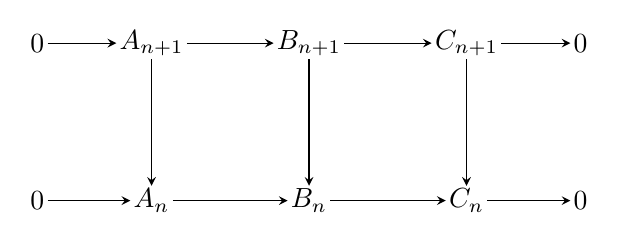
\begin{tikzpicture}[
  baseline=(current bounding box.center),
  every node/.style={inner sep=1pt}
]
  \node (top-zero-left) at (0,1) {$0$};
  \node (top-A) at (1.45,1) {$A_{n+1}$};
  \node (top-B) at (3.45,1) {$B_{n+1}$};
  \node (top-C) at (5.45,1) {$C_{n+1}$};
  \node (top-zero-right) at (6.9,1) {$0$};

  \node (bottom-zero-left) at (0,-1) {$0$};
  \node (bottom-A) at (1.45,-1) {$A_n$};
  \node (bottom-B) at (3.45,-1) {$B_n$};
  \node (bottom-C) at (5.45,-1) {$C_n$};
  \node (bottom-zero-right) at (6.9,-1) {$0$};

  \draw[->,>=stealth] (top-zero-left) -- (top-A);
  \draw[->,>=stealth] (top-A) -- (top-B);
  \draw[->,>=stealth] (top-B) -- (top-C);
  \draw[->,>=stealth] (top-C) -- (top-zero-right);

  \draw[->,>=stealth] (bottom-zero-left) -- (bottom-A);
  \draw[->,>=stealth] (bottom-A) -- (bottom-B);
  \draw[->,>=stealth] (bottom-B) -- (bottom-C);
  \draw[->,>=stealth] (bottom-C) -- (bottom-zero-right);

  \draw[->,>=stealth] (top-A) -- (bottom-A);
  \draw[->,>=stealth] (top-B) -- (bottom-B);
  \draw[->,>=stealth] (top-C) -- (bottom-C);
\end{tikzpicture}

\end{center}
